\documentclass[a4paper, 11pt]{article}
\usepackage[text={170mm,240mm}, left=2cm, top=3cm]{geometry}
\usepackage[czech,linesnumbered,lined,commentsnumbered,ruled]{algorithm2e}
\usepackage[czech,shorthands=off]{babel}
\usepackage[utf8]{inputenc}
\usepackage{times}
\usepackage{algorithmic}
\usepackage{graphicx}
\usepackage{tabu,array,multirow}
\usepackage{pdflscape}
\usepackage{xcolor, picture}
\usepackage{amsmath}
\usepackage[hidelinks]{hyperref}


\renewcommand{\algorithmicensure}{\textbf{Output:}}
\renewcommand{\algorithmicrequire}{\textbf{Input:}}

\begin{document}

%Title page
\begin{titlepage}
    \begin{center}
    \Huge\textsc{Vysoké učení technické v~Brně\\}
        \huge \textsc{Fakulta informačních technologií}\\
        \vspace{\stretch{0.382}}
        \LARGE{Typografie a~publikování\,--\,3. projekt}\\
        \Huge{Tabulky a~obrázky}
        \vspace{\stretch{0.618}}
        
        {\Large 31. března 2024 \hfill Martin Kováčik}
        
    \end{center}
\end{titlepage}

\section{Úvodní strana}\label{1}
Název práce umístěte do zlatého řezu a~nezapomeňte uvést dnešní datum a~vaše jméno a~příjmení.

\section{Tabulky}\label{2}
Pro sázení tabulek můžeme použít buď prostředí\texttt{ tabbing }nebo~prostředí\texttt{ tabular}.
\subsection{Prostředí\texttt{ tabbing}}
Při použití\texttt{ tabbing }vypadá tabulka následovně:
\begin{tabbing}
    \textbf{Ovoce} \hspace{1.6cm} \= \textbf{Cena} \hspace{0.3cm} \= \textbf{Množství}\\
    Jablka  \> 25,90 \> 3 kg\\
    Hrušky  \> 27,40 \> 2,5 kg\\
    Vodní melouny \> 35,-- \> 1 kus\\
\end{tabbing}
Toto prostředí se dá také použít pro sázení algoritmů, ovšem vhodnější je použít prostředí\texttt{ algorithm }nebo \texttt{ algorithm2e }(viz sekce \ref{3}).
\subsection{Prostředí\texttt{ tabular}}
Další možností, jak vytvořit tabulku, je použít prostředí\texttt{ tabular}. Tabulky pak budou vypadat takto\footnote{Kdyby byl problém s\texttt{ cline,} zkuste se podívat třeba sem: \hyperlink{http://www.abclinuxu.cz/tex/poradna/show/325037}{http://www.abclinuxu.cz/tex/poradna/show/325037}.}:
\bigskip
\begin{table}[h]
\begin{center}
    

\catcode`\-=12
\begin{tabular}{|c|c|c|}
\hline
    & \multicolumn{2}{c|}{\textbf{Cena}} \\
    \cline{2-3}    
     \textbf{Měna} & \textbf{nákup} & \textbf{prodej}\\
    \hline
    EUR & 25,475 & 27,045\\
    GBP & 28,835 & 30,705\\
    USD & 22,943 & 24,357\\
\hline
\end{tabular}

\caption{Tabulka kurzů k dnešnímu dni} \label{tabulka1}
\end{center}
\end{table}

\begin{table}[h]
\centering
\catcode`\-=12
\begin{tabular}{|c|c|}
\hline
    $A$ & $\neg A$\\
\hline
    \textbf{P} & N\\
\hline
    \textbf{O} & O\\
\hline
    \textbf{X} & X\\
\hline
    \textbf{N} & P\\
\hline
\end{tabular}
\begin{tabular}{|c|c|c|c|c|c|}
\hline
    \multicolumn{2}{|c|}{\multirow{2}{*}{$A \land B$}} & \multicolumn{4}{|c|}{$B$}\\
    \cline{3-6}
    \multicolumn{2}{|c|}{} & \textbf{P} & \textbf{O} & \textbf{X} & \textbf{N} \\
    \hline
    \multirow{4}{*}{$A$} & \textbf{P} & P & O & X & N \\
    \cline{2-6}
     & \textbf{O} & O & O & N & N\\
     \cline{2-6}
    & \textbf{X} & X & N & X & N\\
    \cline{2-6}
    & \textbf{N} & N & N & N & N\\
\hline
\end{tabular}
\begin{tabular}{|c|c|c|c|c|c|}
\hline
    \multicolumn{2}{|c|}{\multirow{2}{*}{$A \lor B$}} & \multicolumn{4}{|c|}{$B$}\\
    \cline{3-6}
    \multicolumn{2}{|c|}{} & \textbf{P} & \textbf{O} & \textbf{X} & \textbf{N} \\
    \hline
    \multirow{4}{*}{$A$} & \textbf{P} & P & P & P & P \\
    \cline{2-6}
     & \textbf{O} & P & O & P & O\\
     \cline{2-6}
    & \textbf{X} & P & P & X & X\\
    \cline{2-6}
    & \textbf{N} & P & O & X & N\\
\hline
\end{tabular}
\begin{tabular}{|c|c|c|c|c|c|}
\hline
    \multicolumn{2}{|c|}{\multirow{2}{*}{$A \rightarrow B$}} & \multicolumn{4}{|c|}{$B$}\\
    \cline{3-6}
    \multicolumn{2}{|c|}{} & \textbf{P} & \textbf{O} & \textbf{X} & \textbf{N} \\
    \hline
    \multirow{4}{*}{$A$} & \textbf{P} & P & O & X & N \\
    \cline{2-6}
     & \textbf{O} & P & O & P & O\\
     \cline{2-6}
    & \textbf{X} & P & P & X & X\\
    \cline{2-6}
    & \textbf{N} & P & P & P & P\\
\hline
\end{tabular}

\caption{Protože Kleeneho trojhodnotová logika už je \uv{zastaralá}, uvádíme si zde příklad čtyřhodnotové logiky} \label{tabulka2}
\end{table}

\bigskip
\pagebreak

\section{Algoritmy}\label{3}

Pokud budeme chtít vysázet algoritmus, můžeme použít prostředí\texttt{ algorithm\footnote{Pro nápovědu, jak zacházet s~prostředím\texttt{ algorithm,} můžeme zkusit tuhle stránku: \\
\hyperlink{http://ftp.cstug.cz/pub/tex/CTAN/macros/latex/contrib/algorithms/algorithms.pdf}{http://ftp.cstug.cz/pub/tex/CTAN/macros/latex/contrib/algorithms/algorithms.pdf.} }} nebo\texttt{ algorithm2e\footnote{Pro\texttt{ algorithm2e }zase tuhle: \hyperlink{http://ftp.cstug.cz/pub/tex/CTAN/macros/latex/contrib/algorithm2e/doc/algorithm2e.pdf}{http://ftp.cstug.cz/pub/tex/CTAN/macros/latex/contrib/algorithm2e/doc/algorithm2e.pdf.} }}.
Příklad použití prostředí\texttt{ algorithm2e }viz Algoritmus \ref{algoritmus}.

\vspace{0.95em}

\begin{algorithm} \label{algoritmus}
    \algsetup{indent=2em}
    \begin{algorithmic}[1]
    \REQUIRE $(X_{t-1},u_{t},z_{t})$
    \ENSURE $X_{t}$
    \vspace{0.5em}
    \STATE $\overline{X_{t}}=X_{t}=0$
    \FOR{$k=1$ to $M$}
        \STATE $x_{t}^{[k]}=$\emph{ sample\_motion\_model}$(u_{t},x_{t-1}^{[k]})$
        \STATE $\omega_{t}^{[k]}=$\emph{ measurement\_model}$(z_{t},x_{t}^{[k]},m_{t-1})$
        \STATE $m_{t}^{[k]}=updated\_occupancy\_grid(z_{t},x_{t}^{[k]},m_{t-1}^{[k]})$
        \STATE $\overline{X_{t}} = \overline{X_{t}} + \langle x_{x}^{[m]},\omega_{t}^{[m]} \rangle$
    \ENDFOR
    \FOR{$k=1$ to $M$}
        \STATE draw $i$ with probability $\approx \omega_{t}^{[i]}$
        \STATE add $\langle x_{x}^{[k]},m_{t}^{[k]} \rangle$ to $X_{t}$
    \ENDFOR
    \RETURN $X_{t}$

    \end{algorithmic}
        \caption{\normalsize{\textsc{Fast}SLAM}}
\end{algorithm}

\section{Obrázky} \label{4}
Do našich článků můžeme samozřejmě vkládat obrázky. Pokud je obrázkem fotografie, můžeme klidně použít bitmapový soubor. Pokud by to ale mělo být nějaké schéma nebo~něco podobného, je dobrým zvykem takovýto obrázek vytvořit vektorově.

\begin{figure}[h]
    \centering
    \scalebox{0.4}{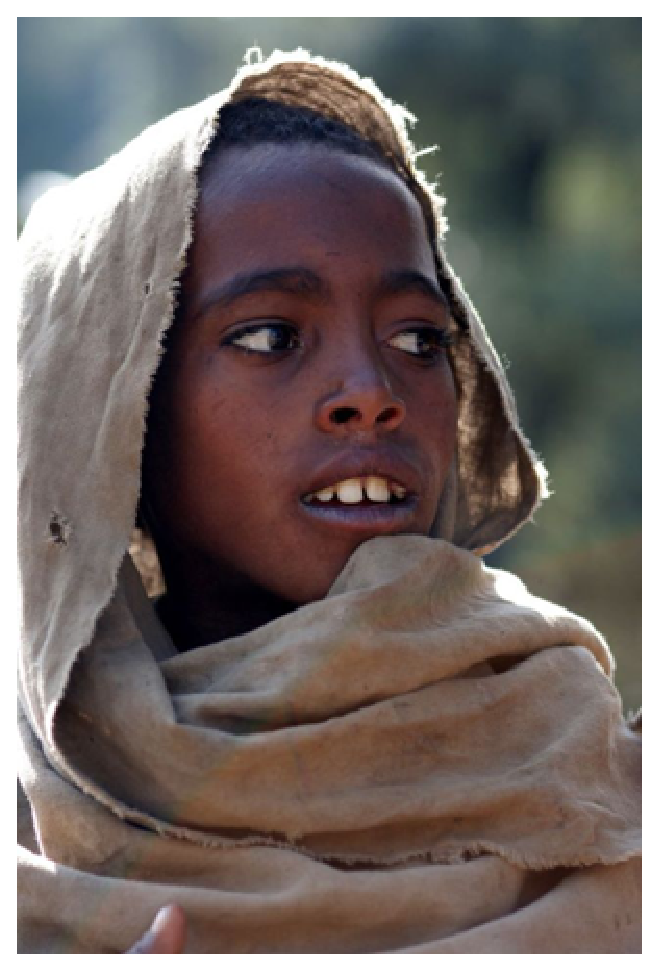
\includegraphics{etiopan.eps}}
    \reflectbox{\scalebox{0.4}{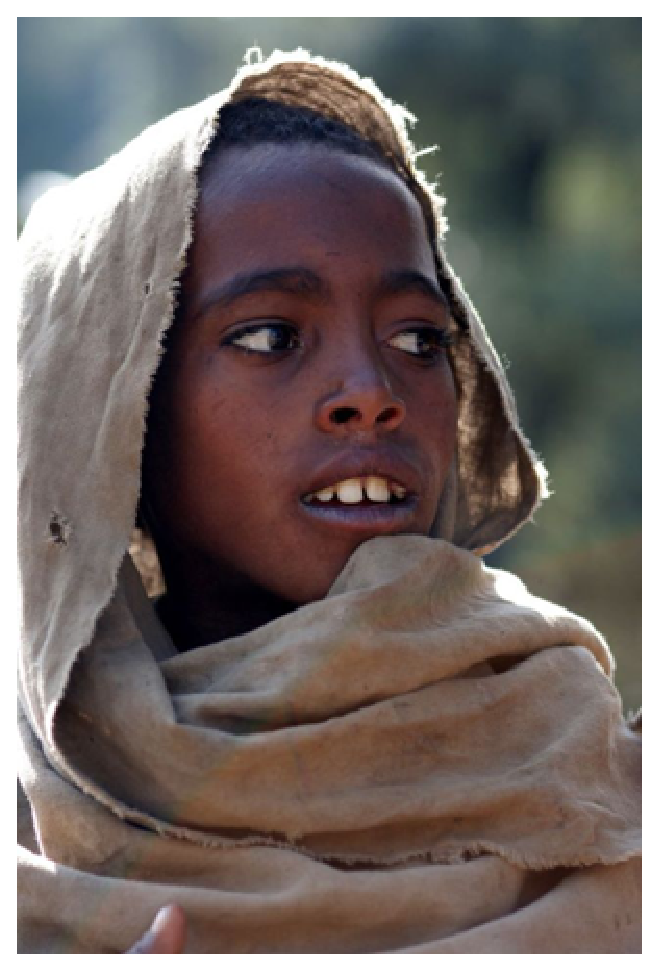
\includegraphics{etiopan.eps}}}
    \caption{Malý Etiopánek a jeho bratříček}\label{Obrazek1}
\end{figure}
\medskip
\pagebreak
Rozdíl mezi vektorovým \dots

\begin{figure}[h]
    \centering
    \scalebox{0.4}{
\includegraphics{oniisan.eps}}
    \caption{Vektorový obrázek}\label{Obrazek2}
\end{figure}
\bigskip
\noindent\dots~a bitmapovým obrázkem

\begin{figure}[h]
    \centering
    \scalebox{0.6}{
\includegraphics{oniisan2.eps}}
    \caption{Bitmapový obrázek}\label{Obrazek3}
\end{figure}
\bigskip
\noindent se projeví například při zvětšení.

Odkazy (nejen ty) na obrázky \ref{Obrazek1}, \ref{Obrazek2} a~\ref{Obrazek3}, na tabulky \ref{tabulka1} a~\ref{tabulka2} a také algoritmus \ref{algoritmus} jsou udělány pomocí křížových odkazů. Pak je ovšem potřeba zdrojový soubor přeložit dvakrát.

Vektorové obrázky lze vytvořit i přímo v \LaTeX{u}, například pomocí prostředí\texttt{ picture.}

\newpage

\begin{landscape}
\begin{figure}
\setlength{\unitlength}{3pt}
    \begin{center}
        \begin{picture}(190, 60)(0,0)
        \setlength\fboxsep{0pt}
        \put(0,0){\framebox(190,95)}
        
        \linethickness{4pt}
        \put(4,13){\line(1,0){182}}
        
        \linethickness{1pt}
        \put(23,13){\line(0,1){34}}
        \put(33.5,13){\line(0,1){13}}
        \put(33.5,26){\line(1,0){34}}
        \put(67.5,26){\line(3,-1){40}}
        \put(41,36.5){\line(1,-1){10.5}}
        \put(41,36.5){\line(1,0){131.7}}
        \put(40.9,36.5){\line(0,1){5.75}}
        \put(40.9,42.25){\line(1,0){131.8}}
        \put(172.7,36.5){\line(0,1){5.75}}
        \put(63.7,42.25){\line(0,1){9.5}}
        \put(23,47){\line(1,0){40.8}}
        \put(63.7,51.75){\line(1,0){53}}
        \put(116.8,42.25){\line(0,1){9.5}}
        \put(116.7,44.1){\line(1,0){46.6}}
        \put(163.3,42.3){\line(0,1){1.8}}
        \put(172.8,13){\line(0,1){8.4}}
        \put(81.4,21.4){\line(1,0){91.4}}
        \put(170.9,21.4){\line(0,1){13.2}}
        \put(71.3,34.7){\line(1,0){99.6}}
        \put(71.3,34.7){\line(0,-1){10}}
        \put(161.5,75.5){\circle{20}}
        
        \end{picture}
        \end{center}
        \caption{Vektorový obrázek moderního bydlení vhodného pro 21. století. (Buď to vytvořte stejný obrázek, anebo nakreslete pomocí picture váš vlastní domov.)}
        \label{obrazek4}
    \end{figure}




    
\end{landscape}


\end{document}